\documentclass[tikz,border=12pt]{standalone}
\usepackage{amsmath}
\usetikzlibrary{arrows.meta,calc}

\begin{document}
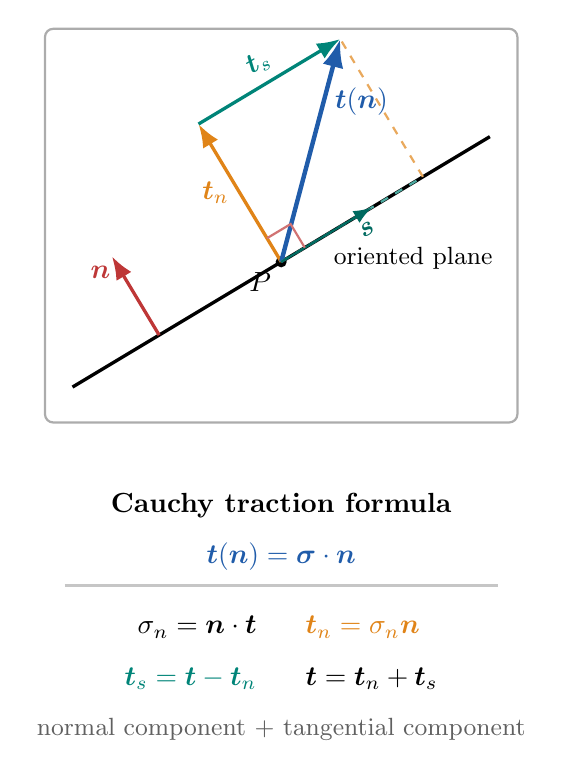
\begin{tikzpicture}[>=Latex,font=\sffamily,thick]
\definecolor{traction}{RGB}{32,92,170}
\definecolor{normal}{RGB}{190,55,55}
\definecolor{normalpart}{RGB}{224,132,24}
\definecolor{shearpart}{RGB}{0,132,120}

% Material neighborhood and an oriented internal plane (line drawing only).
\path[draw=gray!65,rounded corners=3pt]
  (-3.0,-2.0) rectangle (3.0,3);
\draw[very thick] (-2.65,-1.55)--(2.65,1.63)
  node[pos=0.6,below right,font=\small] {oriented plane};

\coordinate (P) at (0,0.04);
\coordinate (N) at (-1.05,1.79);
\coordinate (S) at (1.80,1.12);
\coordinate (T) at (0.75,2.87);

\fill (P) circle (2pt) node[below left] {$P$};

% Unit normal, drawn away from P so it does not overlap the normal traction.
\draw[->,normal,very thick] (-1.55,-0.89)--(-2.15,0.11)
  node[pos=0.80,left] {$\boldsymbol n$};
\draw[->,normalpart,very thick] (P)--(N)
  node[midway,left] {$\boldsymbol t_n$};
\draw[->,shearpart,very thick] (N)--(T)
  node[midway,above,sloped] {$\boldsymbol t_s$};
\draw[->,traction,ultra thick] (P)--(T)
  node[pos=0.72,right] {$\boldsymbol t(\boldsymbol n)$};

% Parallelogram construction.
\draw[dashed,shearpart!70] (P)--(S);
\draw[dashed,normalpart!70] (S)--(T);
\draw[->,shearpart!80!black] (P)--(1.15,0.73)
  node[pos=0.85,below,sloped] {$\boldsymbol s$};

% Right-angle mark between tangent and normal directions.
\draw[normal!70]
  ($(P)+(0.30,0.18)$)--($(P)+(0.12,0.48)$)--($(P)+(-0.18,0.30)$);

% Explanatory equations placed below to keep the figure compact in width.
\begin{scope}[shift={(0,-3.05)}]
  \node[font=\bfseries] at (0,0)
    {Cauchy traction formula};
  \node[traction] at (0,-0.65)
    {$\boldsymbol t(\boldsymbol n)=\boldsymbol\sigma\cdot\boldsymbol n$};
  \draw[gray!45] (-2.75,-1.02)--(2.75,-1.02);
  \node[anchor=east] at (-0.18,-1.55)
    {$\sigma_n=\boldsymbol n\cdot\boldsymbol t$};
  \node[anchor=west,normalpart] at (0.18,-1.55)
    {$\boldsymbol t_n=\sigma_n\boldsymbol n$};
  \node[anchor=east,shearpart] at (-0.18,-2.20)
    {$\boldsymbol t_s=\boldsymbol t-\boldsymbol t_n$};
  \node[anchor=west] at (0.18,-2.20)
    {$\boldsymbol t=\boldsymbol t_n+\boldsymbol t_s$};
  \node[font=\small,gray!75!black] at (0,-2.85)
    {normal component $+$ tangential component};
\end{scope}

\end{tikzpicture}
\end{document}
